%% Based on a TeXnicCenter-Template by Tino Weinkauf.
%%%%%%%%%%%%%%%%%%%%%%%%%%%%%%%%%%%%%%%%%%%%%%%%%%%%%%%%%%%%%

%%%%%%%%%%%%%%%%%%%%%%%%%%%%%%%%%%%%%%%%%%%%%%%%%%%%%%%%%%%%%
%% HEADER
%%%%%%%%%%%%%%%%%%%%%%%%%%%%%%%%%%%%%%%%%%%%%%%%%%%%%%%%%%%%%
\documentclass[a4paper,twoside,10pt]{report}
% Alternative Options:
%	Paper Size: a4paper / a5paper / b5paper / letterpaper / legalpaper / executivepaper
% Duplex: oneside / twoside
% Base Font Size: 10pt / 11pt / 12pt


%% Language %%%%%%%%%%%%%%%%%%%%%%%%%%%%%%%%%%%%%%%%%%%%%%%%%
\usepackage[USenglish]{babel} %francais, polish, spanish, ...
\usepackage[T1]{fontenc}
\usepackage[ansinew]{inputenc}

\usepackage{lmodern} %Type1-font for non-english texts and characters


%% Packages for Graphics & Figures %%%%%%%%%%%%%%%%%%%%%%%%%%
\usepackage{graphicx} %%For loading graphic files
%\usepackage{subfig} %%Subfigures inside a figure
%\usepackage{pst-all} %%PSTricks - not useable with pdfLaTeX

%% Please note:
%% Images can be included using \includegraphics{Dateiname}
%% resp. using the dialog in the Insert menu.
%% 
%% The mode "LaTeX => PDF" allows the following formats:
%%   .jpg  .png  .pdf  .mps
%% 
%% The modes "LaTeX => DVI", "LaTeX => PS" und "LaTeX => PS => PDF"
%% allow the following formats:
%%   .eps  .ps  .bmp  .pict  .pntg


%% Math Packages %%%%%%%%%%%%%%%%%%%%%%%%%%%%%%%%%%%%%%%%%%%%
\usepackage{amsmath}
\usepackage{amsthm}
\usepackage{amsfonts}


%% Line Spacing %%%%%%%%%%%%%%%%%%%%%%%%%%%%%%%%%%%%%%%%%%%%%
%\usepackage{setspace}
%\singlespacing        %% 1-spacing (default)
%\onehalfspacing       %% 1,5-spacing
%\doublespacing        %% 2-spacing


%% Other Packages %%%%%%%%%%%%%%%%%%%%%%%%%%%%%%%%%%%%%%%%%%%
\usepackage{a4wide} %%Smaller margins = more text per page.
%\usepackage{fancyhdr} %%Fancy headings
%\usepackage{longtable} %%For tables, that exceed one page


%%%%%%%%%%%%%%%%%%%%%%%%%%%%%%%%%%%%%%%%%%%%%%%%%%%%%%%%%%%%%
%% Remarks
%%%%%%%%%%%%%%%%%%%%%%%%%%%%%%%%%%%%%%%%%%%%%%%%%%%%%%%%%%%%%
%
% TODO:
% 1. Edit the used packages and their options (see above).
% 2. If you want, add a BibTeX-File to the project
%    (e.g., 'literature.bib').
% 3. Happy TeXing!
%
%%%%%%%%%%%%%%%%%%%%%%%%%%%%%%%%%%%%%%%%%%%%%%%%%%%%%%%%%%%%%

%%%%%%%%%%%%%%%%%%%%%%%%%%%%%%%%%%%%%%%%%%%%%%%%%%%%%%%%%%%%%
%% Options / Modifications
%%%%%%%%%%%%%%%%%%%%%%%%%%%%%%%%%%%%%%%%%%%%%%%%%%%%%%%%%%%%%

%\input{options} %You need a file 'options.tex' for this
%% ==> TeXnicCenter supplies some possible option files
%% ==> with its templates (File | New from Template...).



%%%%%%%%%%%%%%%%%%%%%%%%%%%%%%%%%%%%%%%%%%%%%%%%%%%%%%%%%%%%%
%% DOCUMENT
%%%%%%%%%%%%%%%%%%%%%%%%%%%%%%%%%%%%%%%%%%%%%%%%%%%%%%%%%%%%%
\begin{document}

\pagestyle{empty} %No headings for the first pages.


%% Title Page %%%%%%%%%%%%%%%%%%%%%%%%%%%%%%%%%%%%%%%%%%%%%%%
%% ==> Write your text here or include other files.

%% The simple version:
\title{Databases part 1}
\author{Tran Mingh Tri, Van Looy Ruben, Van de Staey Zimcke}
%\date{} %%If commented, the current date is used.
\maketitle

%% The nice version:
%\input{titlepage} %%You need a file 'titlepage.tex' for this.
%% ==> TeXnicCenter supplies a possible titlepage file
%% ==> with its templates (File | New from Template...).


%% Inhaltsverzeichnis %%%%%%%%%%%%%%%%%%%%%%%%%%%%%%%%%%%%%%%
%\tableofcontents %Table of contents
%\cleardoublepage %The first chapter should start on an odd page.

\pagestyle{plain} %Now display headings: headings / fancy / ...



%% Chapters %%%%%%%%%%%%%%%%%%%%%%%%%%%%%%%%%%%%%%%%%%%%%%%%%
%% ==> Write your text here or include other files.

%\input{intro} %You need a file 'intro.tex' for this.


%%%%%%%%%%%%%%%%%%%%%%%%%%%%%%%%%%%%%%%%%%%%%%%%%%%%%%%%%%%%%
%% ==> Some hints are following:

\section{Assumptions}\label{hints}


The tax per port is not multivalued, there is only one tax-rate per port (independent from the ship type or other characteristics).\\ \\
We assume that a ship can't have more than one route simultaneously. \\ \\
To uniquely identify SHIPMENT(s) (a weak entity type) with the same shipbroker and customer, we inserted a custom ID that functions as a partial key. The attributes Weight and Volume are not sufficient, since there could exist multiple shipments with the same weight and volume.\\ \\
There is no partial key for the weak entity ROUTE, since two routes with the same ports are considered as one and the same.

\section{ER-diagram}

Still have to adjust margins of the page...

\begin{figure}
	\centering
		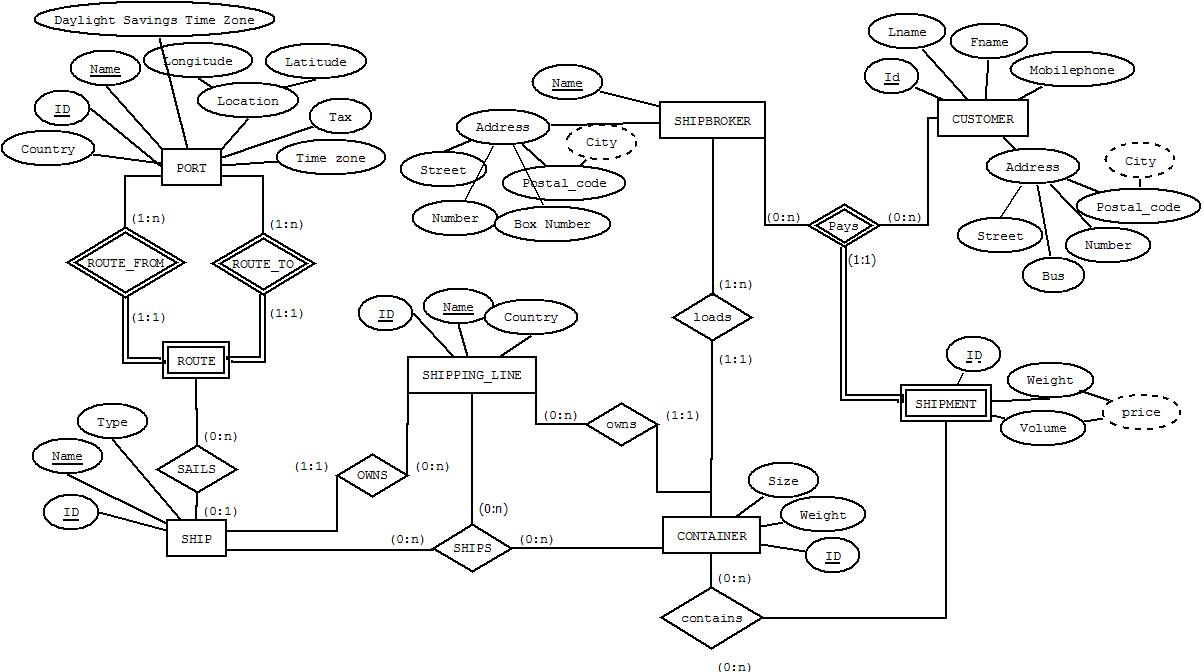
\includegraphics[width=1.00\textwidth]{C:/Users/Zimcke/Documents/GitHub/gegevensbanken/er_diagram.jpg}
	\label{fig:opdracht1}
\end{figure}




%% <== End of hints
%%%%%%%%%%%%%%%%%%%%%%%%%%%%%%%%%%%%%%%%%%%%%%%%%%%%%%%%%%%%%



%%%%%%%%%%%%%%%%%%%%%%%%%%%%%%%%%%%%%%%%%%%%%%%%%%%%%%%%%%%%%
%% BIBLIOGRAPHY AND OTHER LISTS
%%%%%%%%%%%%%%%%%%%%%%%%%%%%%%%%%%%%%%%%%%%%%%%%%%%%%%%%%%%%%
%% A small distance to the other stuff in the table of contents (toc)
\addtocontents{toc}{\protect\vspace*{\baselineskip}}

%% The Bibliography
%% ==> You need a file 'literature.bib' for this.
%% ==> You need to run BibTeX for this (Project | Properties... | Uses BibTeX)
%\addcontentsline{toc}{chapter}{Bibliography} %'Bibliography' into toc
%\nocite{*} %Even non-cited BibTeX-Entries will be shown.
%\bibliographystyle{alpha} %Style of Bibliography: plain / apalike / amsalpha / ...
%\bibliography{literature} %You need a file 'literature.bib' for this.

%% The List of Figures
%%\clearpage
%%\addcontentsline{toc}{chapter}{List of Figures}
%%\listoffigures

%% The List of Tables
%%\clearpage
%%\addcontentsline{toc}{chapter}{List of Tables}
%%\listoftables


%%%%%%%%%%%%%%%%%%%%%%%%%%%%%%%%%%%%%%%%%%%%%%%%%%%%%%%%%%%%%
%% APPENDICES
%%%%%%%%%%%%%%%%%%%%%%%%%%%%%%%%%%%%%%%%%%%%%%%%%%%%%%%%%%%%%
\appendix
%% ==> Write your text here or include other files.

%\input{FileName} %You need a file 'FileName.tex' for this.


\end{document}

